% !TeX root = ../main.tex
\chapter{Introduction}
\section{Residential Shift and Internal Migration}
% <motivating using CDRs to identify internal migration.>
Call Detailed Records (referred to as CDRs hereafter) is a collection of geotagged phone call records (Table \ref{tab:example_cdr}) over a period of time. By looking at individual level, we can trace phone users' geographical appearances with temporal dimension. Based on the spatial patterns distributed on the map, we can estimate their significant locations, such as their residential coordinates and workplace location. Besides, the temporal dimension offers a particularly exciting opportunity: we can identify events of residential shifts, depicting migration flows that were previously impossible to capture at such scale and precision through traditional census-based survey.

\begin{table}[htbp]
\vspace{0.3cm}
\renewcommand{\arraystretch}{1.6}
\setlength{\tabcolsep}{1.9mm}{}
\centering
\scriptsize
\caption{An example of geotagged CDRs}

% \begin{tabular}{>{\centering\arraybackslash}p{1.5cm}>{\centering\arraybackslash}p{1.4cm}>{\centering\arraybackslash}p{2.5cm}>{\centering\arraybackslash}p{2.5cm}>{\centering\arraybackslash}p{1.5cm}>{\centering\arraybackslash}p{1.5cm}>{\centering\arraybackslash}p{1.2cm}}
\begin{tabular}{ccccccc}
\hline

\textbf{Client Number} & \textbf{Duration} & \textbf{Start Time} & \textbf{End Time} & \textbf{Calling Number} & \textbf{Called Number} & \textbf{Cell ID} \\ \hline

66ak2s5v & 62.0 & 2013-08-31 09:32:08 & 2013-08-31 09:33:10 & 66ak2s5v & moyl2k57 & 3649 \\

ltzkksuv & 148.0 & 2013-08-31 09:33:55 & 2013-08-31 09:36:23 & ltzkksuv & hjo0ksut & 3B56 \\

njo45k8v & 46.0 & 2013-08-31 09:36:03 & 2013-08-31 09:36:49 & 8yro82d5 & njo45k8v & 394C \\

\multicolumn{7}{c}{\vdots} \\
\hline
\label{tab:cdr}%
\end{tabular}%

\label{tab:example_cdr}
\end{table}

\vspace{-3em}
\begin{singlespace}
\begin{footnotesize}
\noindent Notes: All phone numbers are anonymized. Cell IDs are the IDs of the telecom base stations handling call events for client numbers, which are either calling numbers or called numbers. We have a dataset which records the geographical coordinates of cell IDs.
\end{footnotesize}
\end{singlespace}

% <elaborating the importance of the topic of internal migration>
This type of human movement is referred to as internal migration, unlike international migration, and it signifies population flow that occurs within a country. Internal migration is a phenomenon that has captured economists' attention for over a century. This strand of literature often involves modeling migration decisions (\cite{hunt2004north}, \cite{espindola2006harris}, \cite{wang2023job}) or inspecting the impacts of migration on the destination region (\cite{boustan2010effect}, \cite{bryan2019aggregate}, \cite{imbert2022migrants}).

% <explaining our contribution> <note that what we have done differently will be elaborated in other section>
CDRs are collected from Sichuan province, China, and the sample periods covers from August 2013 to May 2014. In China, most of the discussion on internal migration is concentrated on the rural-urban migration on the prefecture level with the reason of finding better jobs or seeking education opportunities. Nonetheless, we don't stress on any particular context of internal migration and focus on the detection of residential shifts and their influences on human behaviors.

We make the contribution in a methodological sense by identifying large-scale inter-prefecture migration flows through novel data sources. Specifically, we employ CDRs and develop a systematic pipeline with two stages to identify people changing their residential locations, revealing the internal migration flows across prefectures. Furthermore, we identify effects of residential shift on human mobility and mobile communication patterns through a staggered DiD design designed by \cite{callaway2021difference}, which allows staggered treatment, variable treatment timing and anticipation of treatment.

Utilizing CDRs to identify internal migration flow has several advantages. First, CDRs capture mobility patterns for virtually all mobile phone users in a region, including populations often underrepresented in conventional surveys such as transient residents, undocumented individuals, and those reluctant to participate in formal governmental data collection. Second, CDRs provide continuous temporal coverage rather than the periodic snapshots offered by censuses, enabling the detection of short-term or seasonal relocations. Third, this approach is also cost-effective compared to the large amount of money and human resources devoted to completing a census, as telecommunication companies automatically collect these phone records for billing purposes.

\section{The Effects of Residential Shift}
CDRs are ubiquitous and extensively utilized in human mobility research (\cite{gonzalez2008understanding}, \cite{song2010limits}, \cite{wesolowski2016connecting}) and social network analysis (\cite{onnela2007structure}, \cite{cho2011friendship}, \cite{referral_effect_2023aer}). Most of the existing works are correlation studies, however, we want to examine the causal effect of residential shift on change in mobility patterns and mobile communication behaviors through a staggered DiD design.

By employing different kinds of auxiliary data sources with our identification approach on residential shifts, we can potentially quantify various effects arising from the residential shift. In this study, we present two illustrative examples that examine the impacts of residential relocation on human mobility patterns and mobile communication behaviors. To characterize the patterns of human mobility, we construct three variables: radius of gyration (\cite{gonzalez2008understanding}, \cite{ranjan2012call}, \cite{pappalardo2015returners}), movement entropy (\cite{eagle2010network}, \cite{song2010limits}, \cite{pappalardo2016analytical}) and eccentricity (\cite{yuan2012correlating}, \cite{zhao2019effect}), which seeks to measure the spatial dispersion of travel, the unpredictability of human movement, and how closely the spatial distribution of locations resembles an ellipse, respectively. To have an understanding on what's the meaning of different mobility features' values, please refer to Figure \ref{fig:mobility}. Speaking of mobile communication behavior, we create two types of features, call duration and contact distance, combined with two distinct directions of communication, outgoing and incoming, thereby generating four features.

<display the evolution of causal parameters>

We find that the residential shift leads to a significant positive increases in all mobility and mobile communication features in the beginning of the residential shift. The effecrts on call duration and radius of gyration are extremely short-lived, which vanished within two months after the residential shift. However, the effects on contact distance, movement entropy, and eccentricity behave differently with dramatically increasing in the first month and gradually decreasing in the following months to a even lower level than that prior to the residential shift.


\section{Mobility and Mobile Communication Features}
Whether immigrants are integrated into the destination region is a topic of great interest to policymakers. \cite{voukelatou2021measuring} provides an overview on utilizing CDRs to measure objective well-being on various dimensions, such as job opportunities, socioeconomic development and so on by analyzing mobility and mobile communication behaviors. Therefore, these two groups of features could be used to measure the integration of immigrants into the destination region. To clarify, what we mean by integration is that immigrants going back to the lifestyle before the residential shift, getting used to the new environment. Moving to a new environment, people might change their communication behaviors toward their old friends or their mobility patterns might be substantially different from their old lifestyle. We have confirmed the changes after immigration and found short-term effects, which means they instantly find their own way to adapt to the new environment.

\vspace{0.3cm}
\begin{figure}[h!]
\centering
\caption{Comparison of Mobility Feature Values}
\vspace{0.1cm}

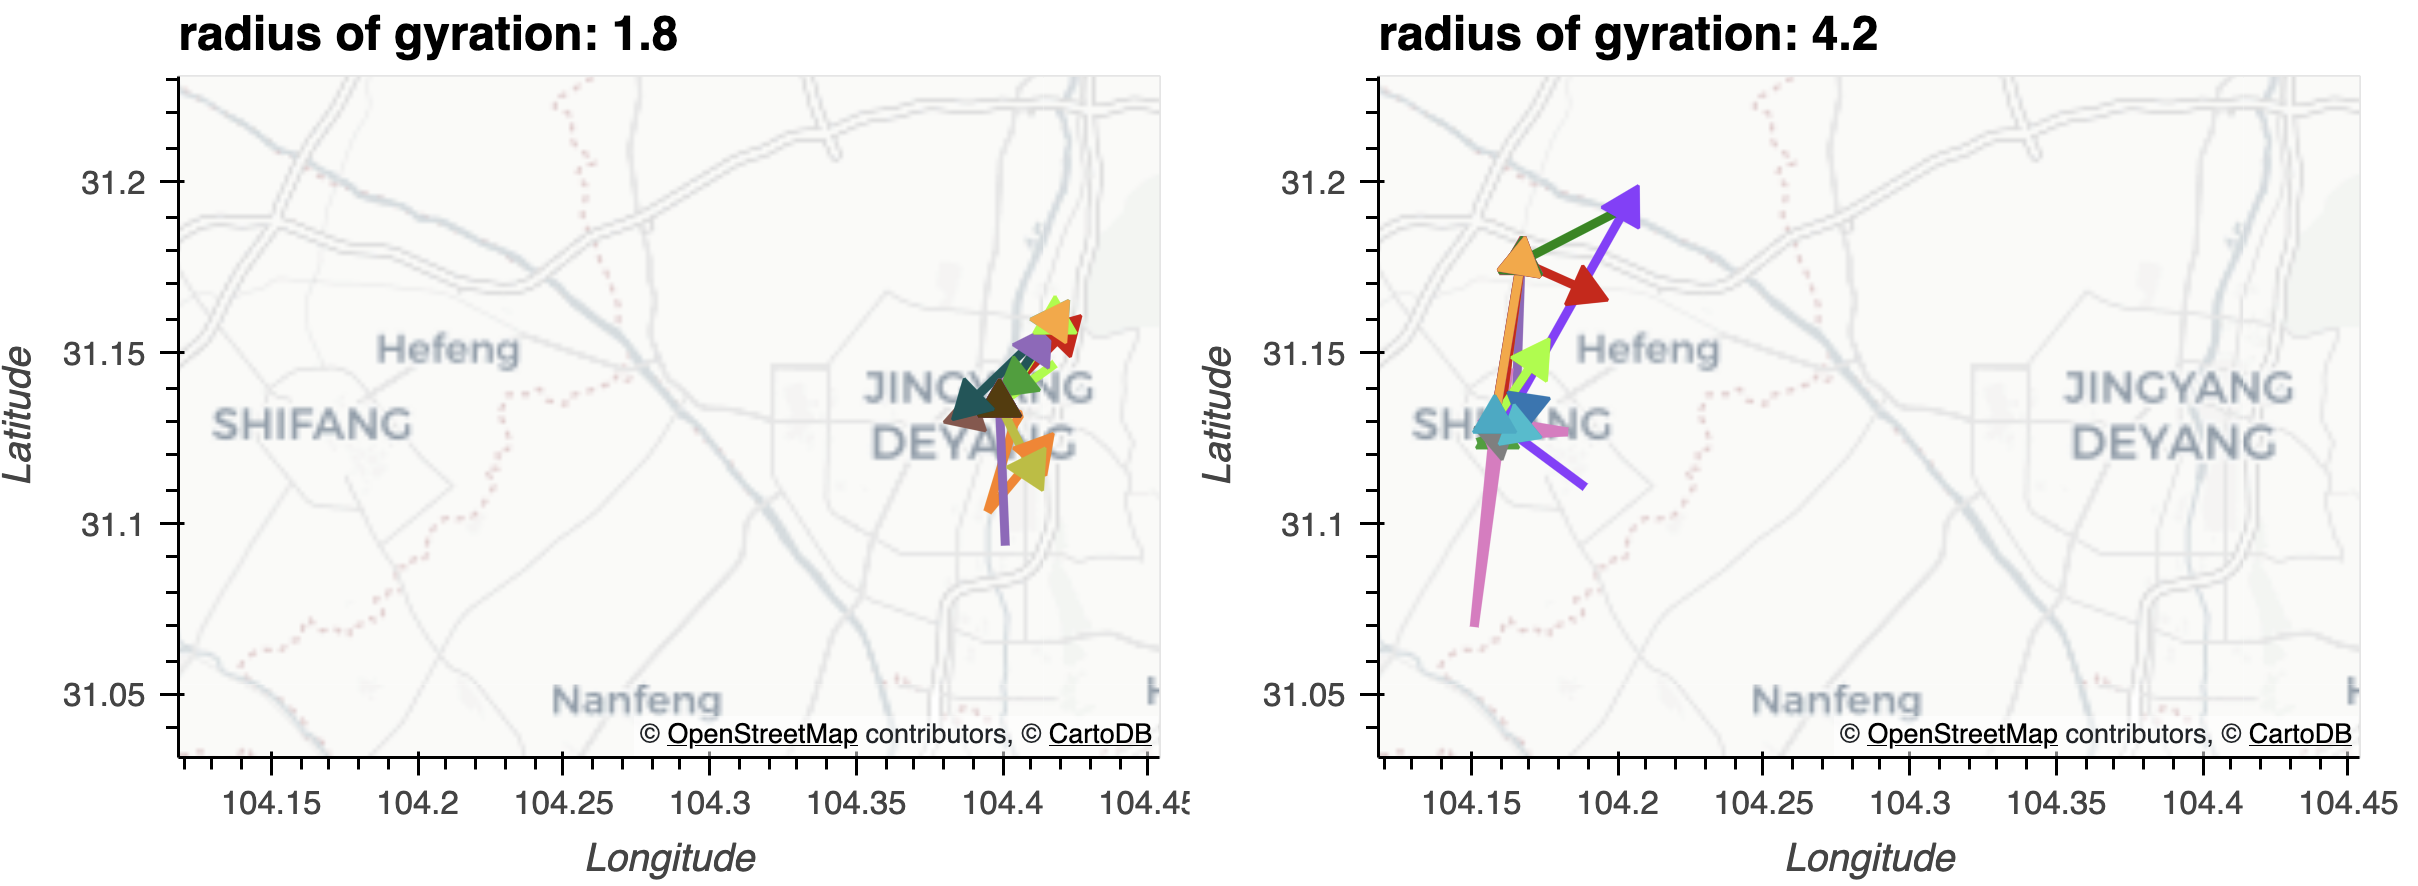
\includegraphics[width=1\textwidth]{figures/rg_compare.png}
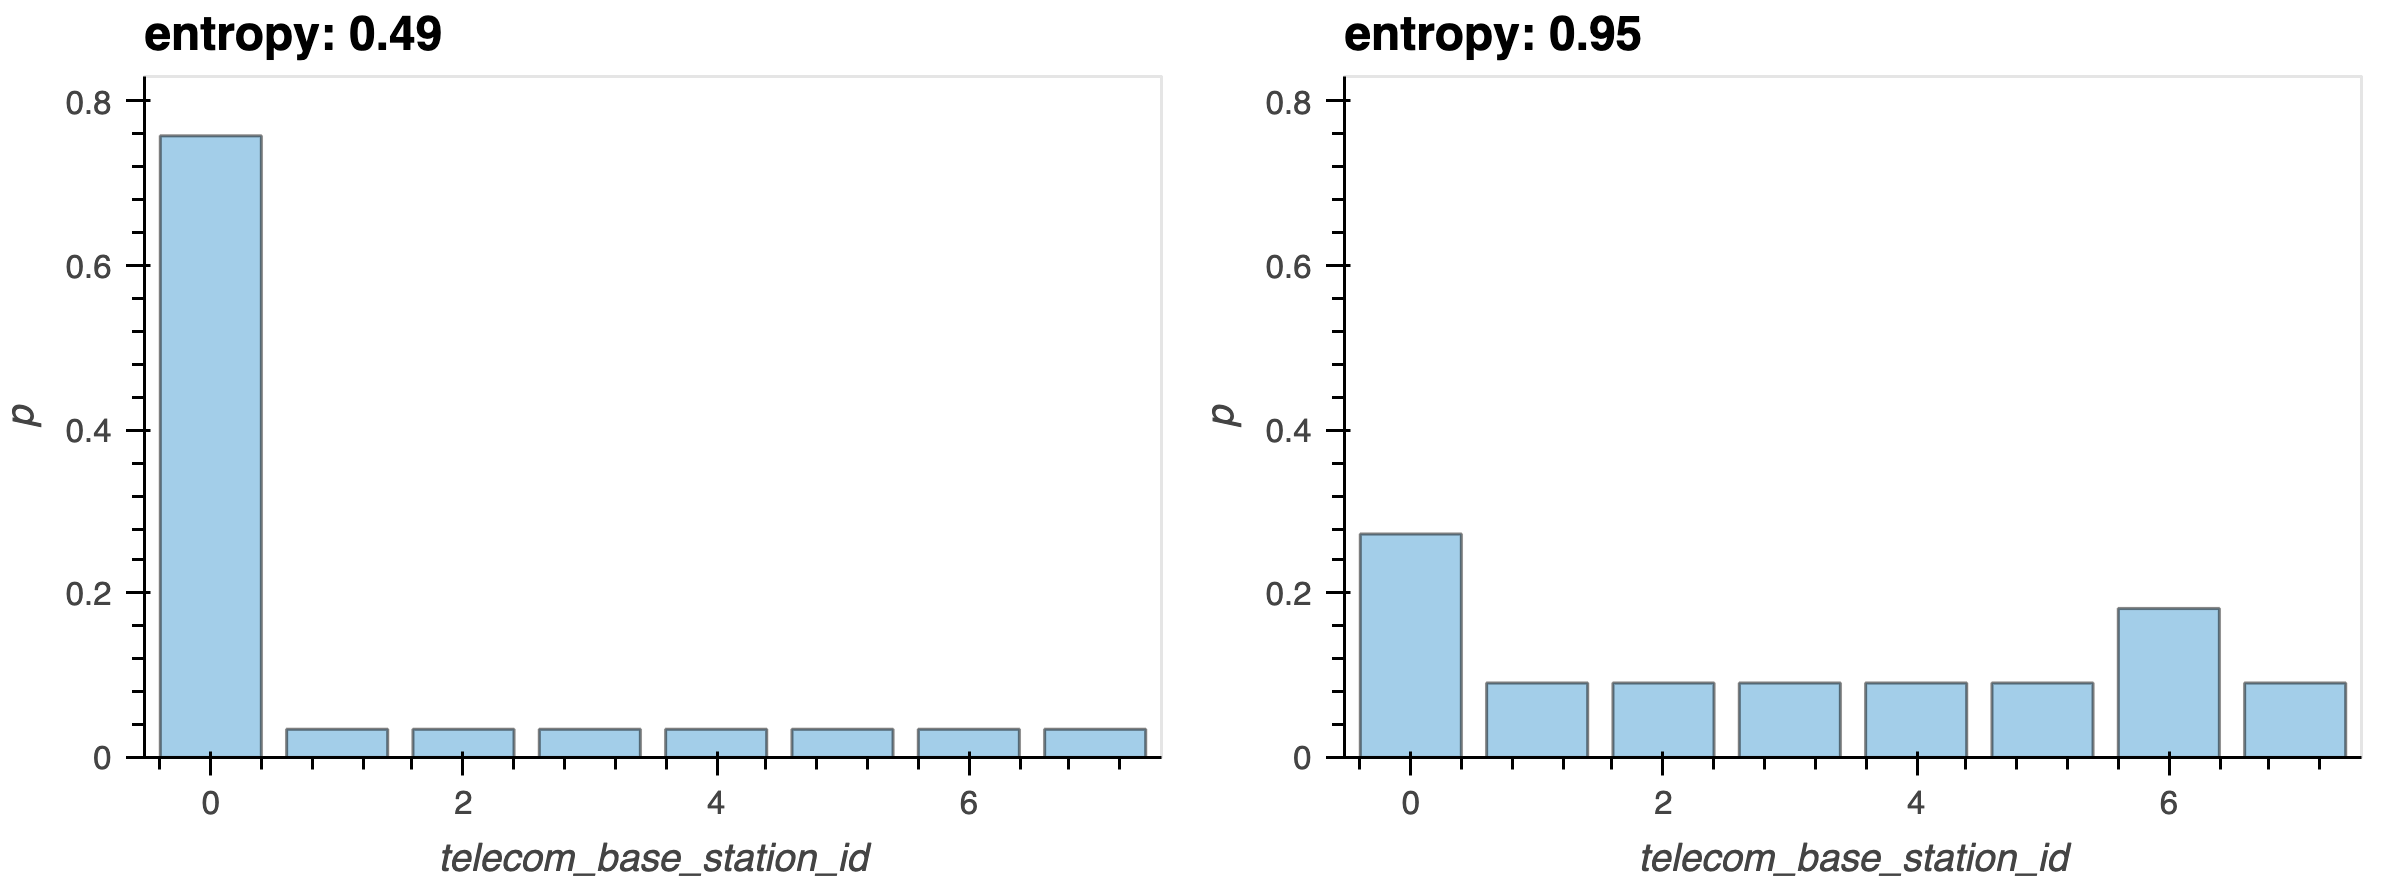
\includegraphics[width=1\textwidth]{figures/entropy_compare.png}
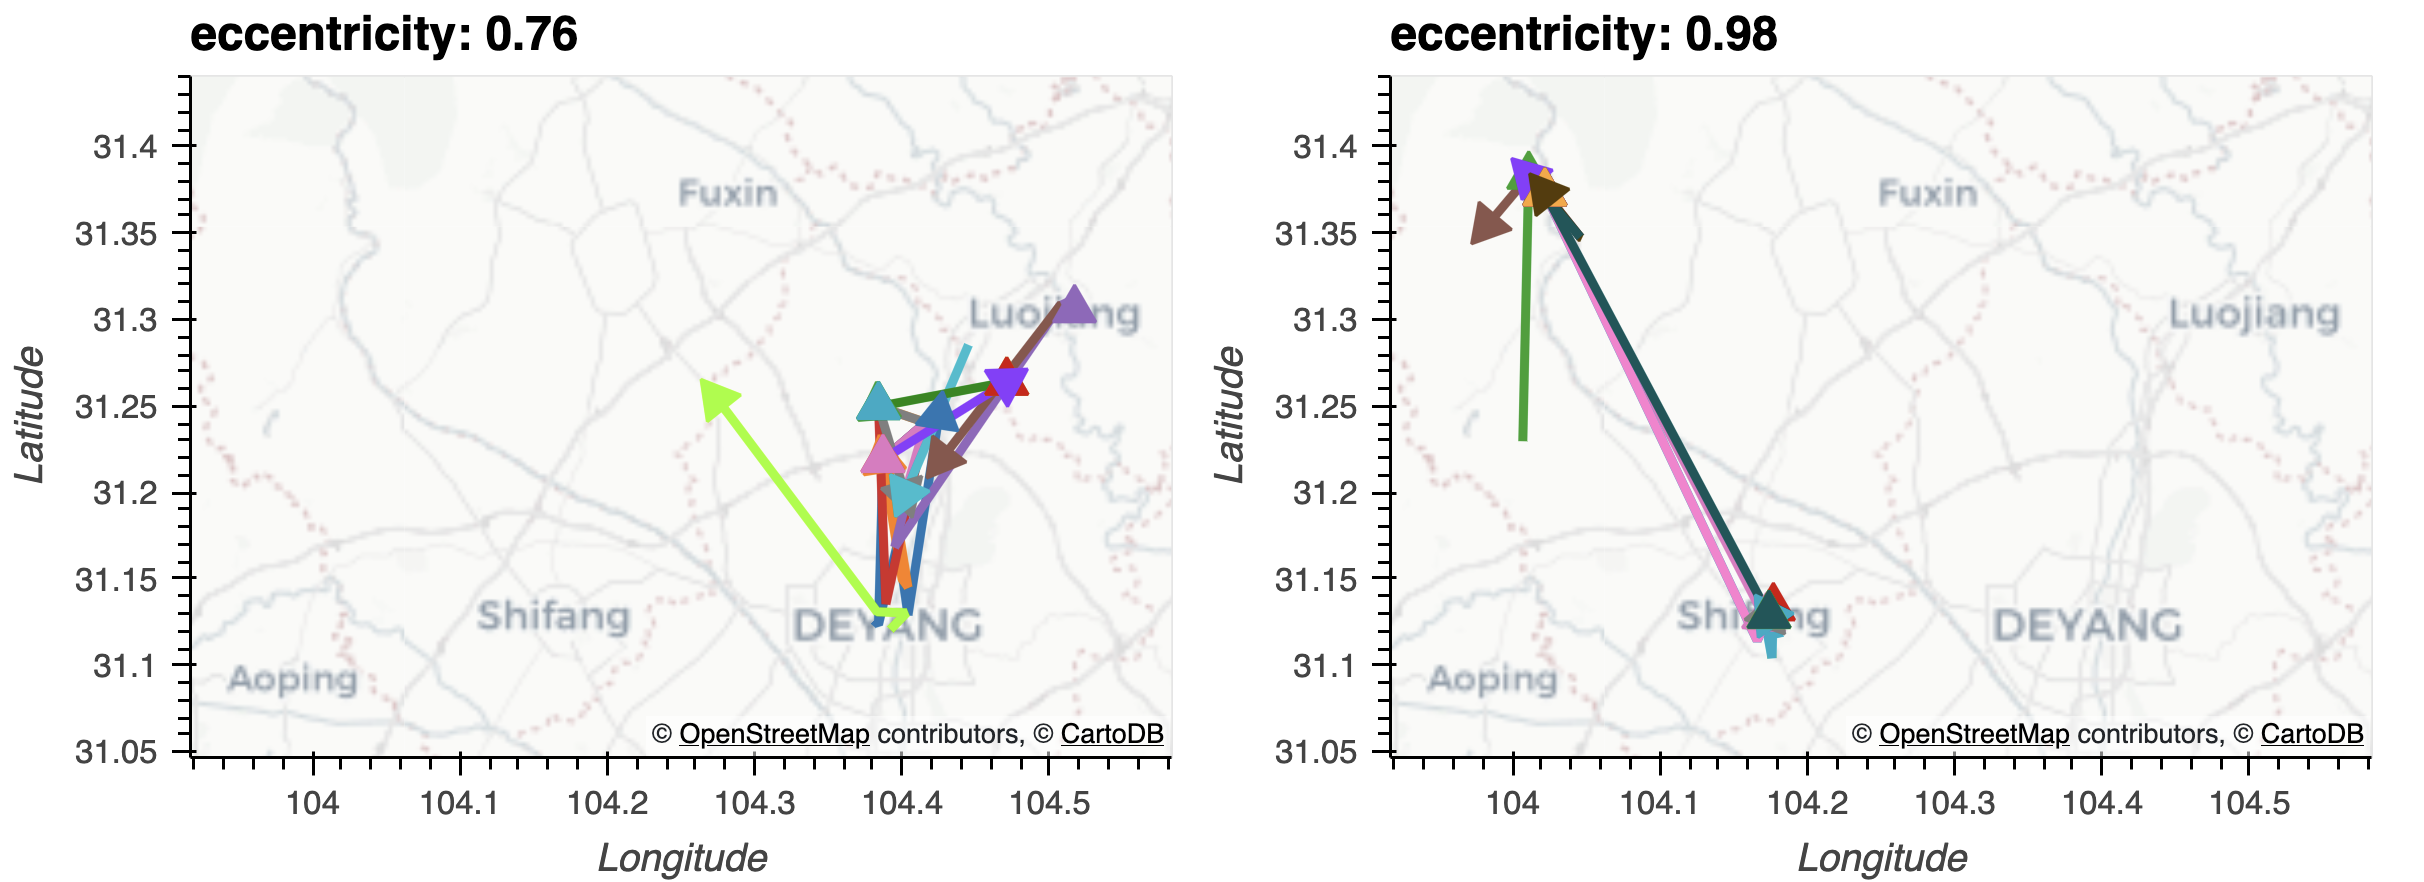
\includegraphics[width=1\textwidth]{figures/ecc_compare.png}

\vspace{0.1cm}
\caption*{Notes:  For radius of gyration and eccentricity, we visualize daily movement trajectories of four phone users throughout August 2013. Regarding entropy, we examine the distribution of telecom base station usage for two phone users during the same period, where the y-axis (p) represents the proportion of total days on which each base station was activated, calculated as the number of days a station served calls divided by the total number of such days across all stations.}
\label{fig:mobility}
\end{figure}

One of the mobile communication network features, the contact distance, captures the average geographical distance between individuals and their contacts, offering insight into the spatial reach of their social interactions. A higher contact distance suggests that a person frequently interacts with others who live far away, which may indicate broader social ties, long-distance relationships, or mobility patterns such as migration or commuting, and as mentioned previously, it shows a significant change after a residential shift. Therefore, we reckon that the contact distance is a good indicator of community integration, providing useful policy implications.

\section{A Novel Approach to Residential Location Estimation}
A critical preliminary step for identifying residential shifts is estimating phone users' home coordinates. It is important to clarify that the coordinates attached to each phone call record don't precisely represent the exact geographical position of either the caller or callee. Rather, they are the coordinates of the telecom base station handling the call, which serve as a spatial approximation for the phone user's position while initiating or receiving phone calls. The approximation is not always accurate due to the routing mechanism, aiming to balance traffic among surrounding telecom base stations.


The routing mechanism brings about two concerns when it comes to estimating residential locations. First, the telecom bases station handling a call event may not always be the closest one (\cite{yuan2012correlating}). Second, even if a user initiates or receives calls at the same place, e.g., at home, the telecom base station serving the call may vary from time to time. Most of the studies estimate home locations by selecting the locations of the telecom base station that handles the call events most frequently over the whole sample period (\cite{cho2011friendship}, \cite{phithakkitnukoon2012socio}), weekly (\cite{referral_effect_2023aer}), or monthly (\cite{phithakkitnukoon2022inferring}) from the nighttime call records.


\vspace{0.3cm}
\begin{figure}[h!]
\centering
\caption{Visualization of Our Proposed Two-Staged Residential Location Estimation}
\vspace{0.1cm}

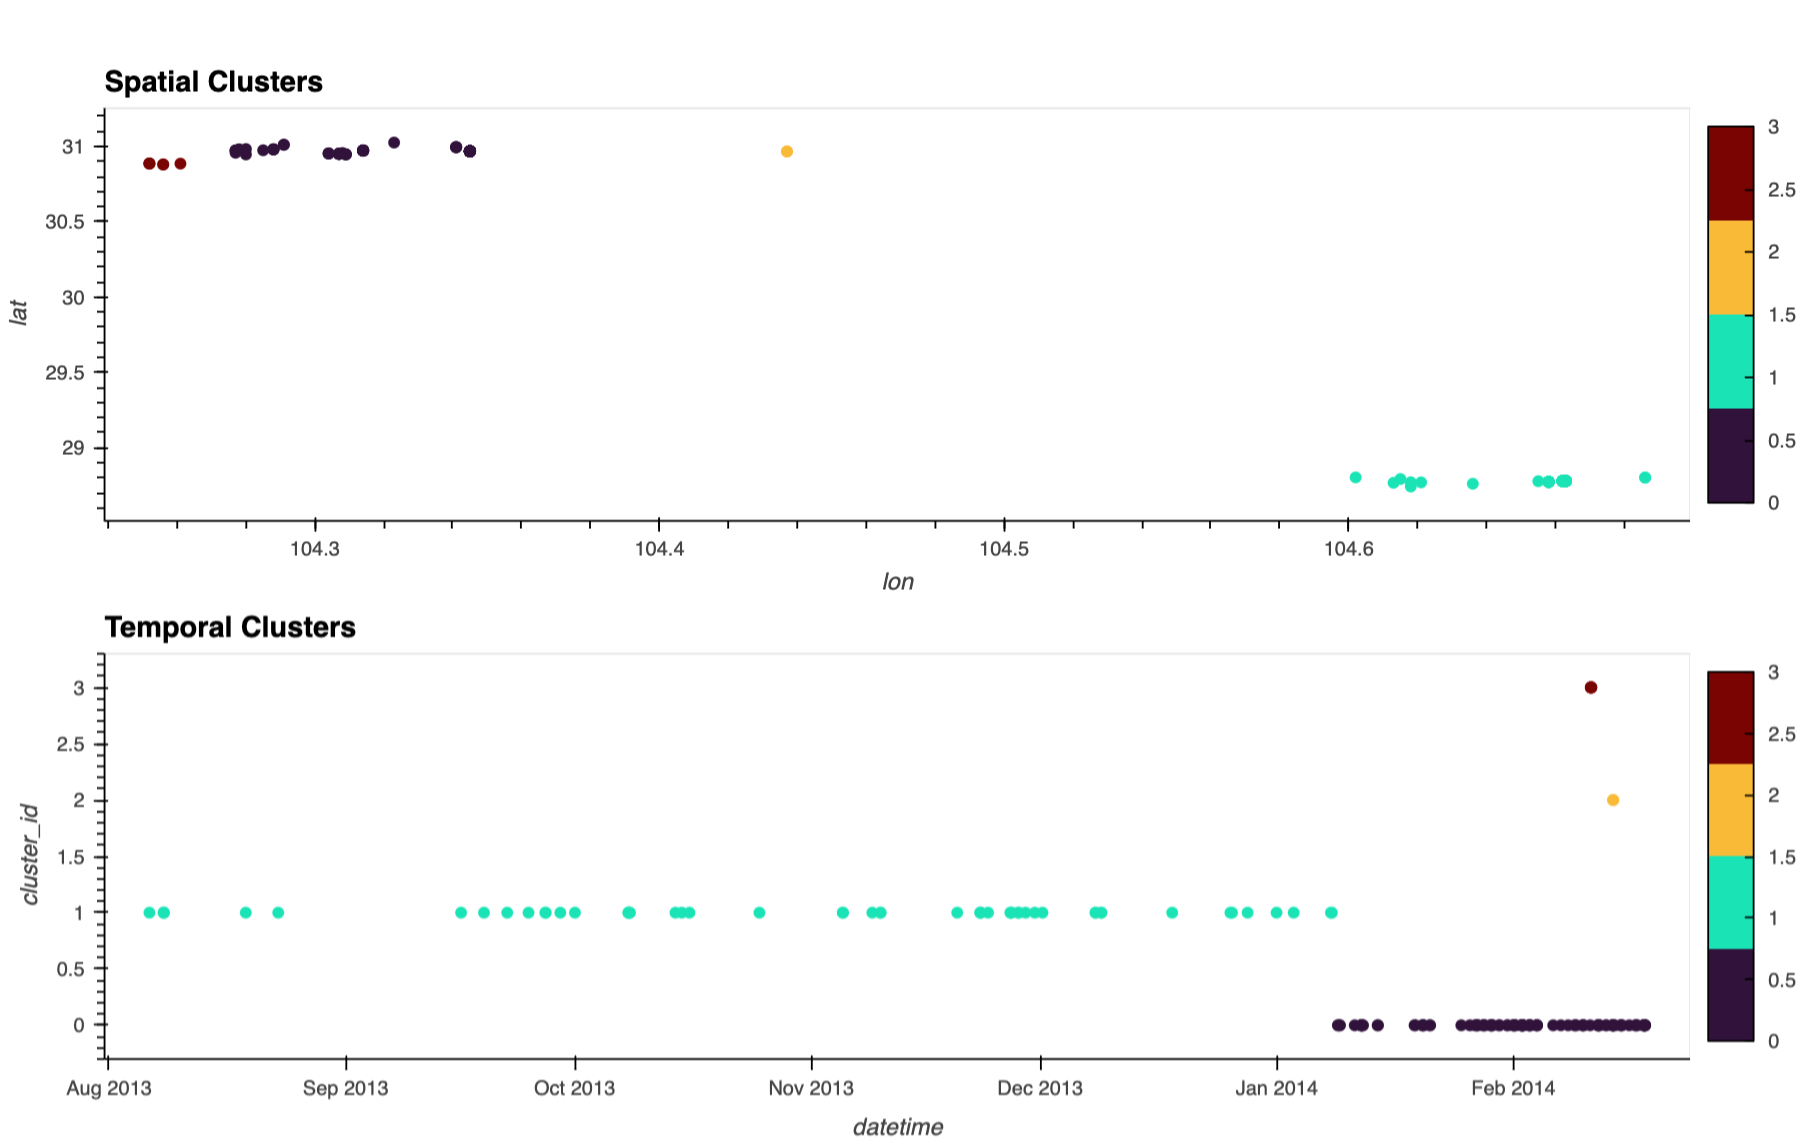
\includegraphics[width=1\textwidth]{figures/cluster_res.png}

\vspace{0.1cm}
\caption*{Notes:  This figure demonstrates one of the phone user's mobility patterns. The upper plot's x and y axis represent the longitude and latitude, respectively. The lower plot shows the temporal span of each cluster where the x axis represents the timestamp and the y axis represents the cluster index. The point is colored by the cluster index.}
\label{fig:cluster}
\end{figure}


This simple approach seems to be acceptable for people who have a large amount of phone call records. However, for those who have limited observations of call events, the simple approach is not reliable. A more robust approach would be running a spatial clustering algorithm over a set of telecom base stations' locations (\cite{isaacman2011identifying}, \cite{yang2014identifying}) . As mentioned, our estimation strategy of residential location encompasses two stages, and the first stage recognizes the clustered patterns and leverage DBSCAN (\cite{ester1996density}), a renowned machine learning algorithm in the clustering domain, to uncover them. For the angle of clustering, what the clustering's goal is to recognize the neighbors of each point. The upper plot of Figure \ref{fig:cluster} visualizes the spatial clustering results where there are four clusters identified and colored by the cluster index.


DBSCAN's flexibility has made it a popular choice for analyzing spatial patterns (\cite{yang2014identifying}, \cite{shi2014density}, \cite{dominguez2017sensing}) and mobile communication behaviors (\cite{karahoca2006comparing}, \cite{jabbar2020fraud}). We inherit this idea, including it in our two-staged approach, which carries the specific goal of identifying residential shifts. Our approach makes this identification feasible by incorporating temporal information following the spatial clustering process. Even more recent developments in significant location inference (\cite{tongsinoot2017exploring}, \cite{luo2020research}) don't explicitly consider the situation where people might change their residential locations.


In the second stage, we implement an extremely simple temporal filtering technique to remove unrepresentative clusters possibly caused by temporary visits or anomalous cases. The remaining clusters are well-representative home clusters, the centers of which are identified as home locations. Let us elaborate more on the definition of a representative cluster. We define a cluster to be representative if the temporal spans associated with each cluster are non-overlapping. An example can be found in Figure \ref{fig:cluster} where the 0-th cluster (black) doesn't temporally overlap with the 1-st cluster (green) in the lower plot. Therefore, each home cluster should correspond to a separate life period where the person lived in a particular location. Moreover, the identified home clusters are temporally sequential and mutually exclusive--when one residential period ends, the next begins, with no overlap between them. This somehow defines the temporal clusters and creates a clear timeline of residential history where each home cluster represents a distinct "home era" in chronological order.

\section{Detection of Residential Shift through CDRs}
Several studies have already taken advantage of CDRs to identify residential relocation. Although most of the works on home location inference are not designed for detecting home location shifts in that they often estimate one location over the whole sample period. However, we can still apply these approaches on multiple fixed-size time window (\cite{blumenstock2012inferring}, \cite{phithakkitnukoon2022inferring}, \cite{blumenstock2025migration}), e.g., daily, weekly, or monthly, or between two time periods (\cite{lai2019exploring}, \cite{dias2022framework}) and if more than one home location is found, we can consider it as a residential shift. \cite{phithakkitnukoon2022inferring} is the case where they apply the simple approach on each month to detect residential shifts while \cite{dias2022framework} adopt \cite{isaacman2011identifying}'s home location estimation method on January to March 2013 and July to September 2013, respectively. This strategy for inferring residential shift requires several predefined parameters, such as the minimum time span of each residential location to exclude short-term visits or distance threshold to define the separation of two home locations. Hence, a heavy procedure of sensitive analysis is required to select the appropriate parameters.

\cite{buchel2020calling} also utilize CDRs to identify residential shift and benefits from high-quality data billing addresses, making residential estimation extremely precise and identification of migrants is simply based on whether individuals change their residential locations. However, as such data is not available in most scenarios, thereby failing to be widely applicable.

\cite{chi2020general} is a closely related work. They abandon the first stage by clustering coordinates of telecom base stations if they are in the same administrative district. Furthermore, they apply clustering algorithm on time axis for a district to identify contiguous segments and further merge segments if no other segments from the other district are found. At the last step, they allow the overlapping of segments from different districts to form home locations at different periods. Our two-stage approach not only provides finer spatial resolution but also is simpler and more rigorous. It is simpler due to the removal of temporal clustering and segment merging, and more rigorous due to the prohibition of overlapping segments from different districts.

Our approach stands out for being universal, efficient, and comprehensive. Our approach relies solely on CDRs, requiring no additional information. Sensitivity analysis becomes unnecessary as there is only one parameter, maximum distance between two points, which can be reasonably assigned between 5 to 10 km. Furthermore, we simply unveil the inherent spatial-temporal patterns through unsupervised learning.

\section{The Effects of Smartphone Adoption}
